\documentclass[11pt, a4paper]{article}

\usepackage[utf8]{inputenc}
\usepackage[T1]{fontenc}
\usepackage{amsmath, amssymb, amsfonts}
\usepackage{graphicx}
\usepackage[margin=1in]{geometry}
\usepackage{hyperref}
\usepackage[numbers, sort&compress]{natbib}
\usepackage{booktabs}
\usepackage{siunitx}
\usepackage{caption}
\usepackage{float}
\usepackage{xcolor}

\title{\textbf{Literature-Informed Selective Pulse Primitives for Dispersive cQED}}
\author{cQED Autonomous Research Platform \\ Shyam Shankar Quantum Circuits Group}
\date{\today}

\begin{document}

\maketitle

\begin{abstract}
Selective number-resolved qubit control is the operational core behind both selective qubit rotation (SQR) and selective number-dependent arbitrary phase (SNAP) gates in dispersive circuit QED. The consolidated SQR and hybrid-control studies in this repository relied on those primitives, but they did not yet contain one pulse-level reference study tying the literature pulse prescriptions to a validated, noise-aware dataset under the repository's standard cQED parameters. This work fills that gap using $\omega_q/2\pi=\SI{6.150}{GHz}$, $\omega_c/2\pi=\SI{5.241}{GHz}$, $\alpha/2\pi=\SI{-255}{MHz}$, $\chi/2\pi=\SI{-2.84}{MHz}$, $\chi'/2\pi=\SI{-21}{kHz}$, and $K/2\pi=\SI{-28}{kHz}$.

We implement literature-backed number-selective pulses through the normal \texttt{cqed\_sim} compilation and simulation path: Gaussian and flat-top selective qubit pulses for SQR, the two-selective-$\pi$ geometric SNAP sequence, and noisy replay with representative transmon relaxation, dephasing, and storage thermal occupation. The central results are: (i) closed-system cphase-SQR fidelity reaches $0.999999$ for the Gaussian family and $0.999991$ for the cosine-squared family near $|\chi|T/2\pi=3$; (ii) once noise is included, the best practical SQR point shifts to a shorter flat-top Gaussian pulse at $|\chi|T/2\pi=1$, with average relaxed-fidelity $0.9903$; and (iii) the best SNAP point is a flat-top Gaussian sequence with two $\pi$ pulses of duration \SI{0.775}{\micro s} each, giving closed process fidelity $0.910$ and noisy average state fidelity $0.938$.

Validation confirms that the results are stable under a finer \SI{1}{ns} time step and an increased cavity cutoff, and that the optimized durations remain consistent with the number-resolution conditions reported in the literature. The resulting dataset provides a reusable pulse reference for downstream SQR, SNAP, and hybrid-control studies.
\end{abstract}

\section{Introduction}

Dispersive circuit QED enables control primitives whose action depends on the cavity photon number because the qubit transition frequency is shifted by the dispersive interaction~\cite{koch2007transmon,blais2021circuit}. Two of the most important examples are selective qubit rotation (SQR), which addresses one Fock manifold of the qubit, and selective number-dependent arbitrary phase (SNAP), which returns the ancilla to its original state while imprinting a cavity phase on a chosen Fock component~\cite{heeres2015snap,krastanov2015universal,heeres2017logical}. These gates are central to bosonic error-correction experiments, but their practical performance depends on a tradeoff between spectral selectivity and decoherence.

The existing consolidated studies in this repository already established that cphase-SQR is the natural benchmark target for SQR and that hybrid libraries combining SNAP-like and native dispersive primitives are attractive for local cavity control~\cite{heeres2017logical}. What was missing was a pulse-level reference pass that starts from the literature prescriptions themselves, implements them with the local simulation stack, and re-optimizes them under the repository's standard Hamiltonian and noise parameters.

This study addresses that missing layer. It uses the literature pulse definitions for selective Gaussian and flat-top qubit drives, plus the original two-$\pi$ geometric SNAP construction, then numerically optimizes those families and replays them under noise. The remainder of the paper presents the shared Hamiltonian and pulse conventions, the optimized SQR and SNAP results, the validation checks, and a concrete handoff for future upstreaming and device-calibrated follow-up.

\paragraph{Experiment-facing question.}
The practical question is which literature pulse an experimentalist should actually calibrate first on a typical dispersive device. We therefore frame the study around decisions that matter in the lab: when a shorter selective pulse is worth the extra spectral spillover, when SNAP's longer sequence cost is justified by the need for exact cavity phase control, and which pulse family gives the best starting point before device-specific retuning.

\section{System and Methods}

\subsection{Hamiltonian}

The study uses the dispersive transmon-storage Hamiltonian
\begin{equation}
\frac{H}{\hbar} =
\omega_c a^\dagger a +
\omega_q b^\dagger b +
\frac{\alpha}{2} b^{\dagger 2} b^2 +
\chi a^\dagger a\, b^\dagger b +
\frac{\chi'}{2}(a^\dagger a)^2 b^\dagger b +
\frac{K}{2}(a^\dagger a)^2,
\end{equation}
where $a$ is the storage-cavity lowering operator, $b$ is the transmon lowering operator, $\alpha$ is the transmon anharmonicity, $\chi$ is the leading dispersive shift, $\chi'$ is the second-order dispersive correction, and $K$ is the storage self-Kerr.

\subsection{Simulation Parameters}

\begin{table}[H]
\centering
\caption{Nominal system parameters used throughout the study.}
\begin{tabular}{@{} l l l @{}}
\toprule
Parameter & {Value} & Unit \\
\midrule
Qubit frequency $\omega_q/2\pi$ & 6.150 & GHz \\
Storage frequency $\omega_c/2\pi$ & 5.241 & GHz \\
Anharmonicity $\alpha/2\pi$ & -255 & MHz \\
Dispersive shift $\chi/2\pi$ & -2.84 & MHz \\
Second-order dispersive shift $\chi'/2\pi$ & -21 & kHz \\
Storage self-Kerr $K/2\pi$ & -28 & kHz \\
Transmon truncation $n_\mathrm{tr}$ & 3 & levels \\
Storage truncation $n_\mathrm{cav}$ & 7 & Fock states \\
Logical window & $n=0,\ldots,3$ & --- \\
\bottomrule
\end{tabular}
\label{tab:params}
\end{table}

\begin{table}[H]
\centering
\caption{Noise parameters used for the open-system replay.}
\begin{tabular}{@{} l l l @{}}
\toprule
Parameter & Value & Unit \\
\midrule
Transmon $(T_{1,ge}, T_{1,ef})$ & $(50, 25)$ & $\mu$s \\
Qubit $T_\phi$ & 80 & $\mu$s \\
Storage $\kappa/2\pi$ & 1.0 & kHz \\
Storage thermal occupation $n_\mathrm{th}$ & 0.02 & --- \\
Time step $\Delta t$ & 2 & ns \\
\bottomrule
\end{tabular}
\label{tab:noise}
\end{table}

\subsection{Literature Pulse Definitions}

The guiding pulse prescriptions come from three sources. First, the qcMAP protocol uses a number-selective Gaussian qubit pulse and states that the selectivity requirement is $T \gg 1/(2\chi)$, with a Gaussian truncated at $4\sigma$~\cite{leghtas2013qcmap}. Second, the original SNAP experiment constructs the phase gate from two successive number-selective $\pi$ pulses whose relative phase sets the desired cavity phase~\cite{heeres2015snap}. Third, a recent dual-rail cavity-qubit experiment describes the same number-resolved control layer in terms of truncated Gaussian or flat-top selective pulses in the joint photon-number-splitting regime~\cite{degraaf2025dualrail}.

Those prescriptions are mapped into three study-local waveform families:
\begin{itemize}
\item Gaussian selective qubit drive with area normalization and tunable $\sigma/T$.
\item Cosine-squared selective qubit drive as a smooth baseline already used in the consolidated SQR study.
\item Flat-top Gaussian selective qubit drive with Gaussian ramps and a constant central plateau.
\end{itemize}

For SQR, the physical pulse is the same across the strict and cphase-relaxed targets; ``ConditionalPhaseSQR'' in this repository is therefore treated as a relaxed target metric rather than a distinct waveform. For SNAP, we implement the geometric sequence as two selective $\pi$ pulses on the same manifold with the second pulse phase shifted by $\pi-\theta_n$~\cite{heeres2015snap}.

\subsection{Computational Approach}

All pulse replay uses \texttt{cqed\_sim}'s standard pulse pipeline: study-local pulse definitions produce \texttt{Pulse} objects, which are compiled by \texttt{SequenceCompiler} and propagated with \texttt{prepare\_simulation(...)} and \texttt{NoiseSpec}~\cite{cqed_sim}. We intentionally do \emph{not} replace the simulator; the only study-local addition is the missing pulse-builder layer for SNAP and literature-style selective flat-top pulses.

The optimization itself is a structured grid search over pulse duration, envelope shape parameter, and a small amplitude renormalization factor. For SQR the primary closed-system metric is the branch-averaged cphase-relaxed fidelity used by the consolidated SQR study, while the noisy metric is the average fidelity over basis and branch-local superposition probe states. For SNAP the closed metric is cavity-process fidelity on the qubit-ground logical manifold, and the noisy metric is the average fidelity over basis and pair-superposition cavity states.

\section{Results}

\subsection{Selective Qubit Rotation}

The closed-system SQR results recover the same qualitative hierarchy seen in the consolidated SQR study, but now with literature-driven pulse families and explicit amplitude re-optimization. Gaussian and cosine-squared selective pulses both peak near $|\chi|T/2\pi=3$, reaching branch-averaged cphase fidelities $0.9999985$ and $0.9999913$, respectively. The flat-top Gaussian family reaches a comparable closed optimum $0.9993998$ at a shorter $|\chi|T/2\pi=2.2$.

The more important practical result appears after noisy replay. The best noisy SQR point is not one of the longest, most selective pulses: it is a flat-top Gaussian pulse at $|\chi|T/2\pi=1.0$, with total duration \SI{0.352}{\micro s}, closed cphase fidelity $0.9954$, and noisy average state fidelity $0.9903$. The best noisy Gaussian and cosine-squared points remain excellent, $0.9898$ and $0.9892$, but both require longer durations (\SI{0.458}{\micro s} and \SI{0.599}{\micro s}, respectively). Figure~\ref{fig:sqr_scan} summarizes the full family scan.

\begin{figure}[H]
  \centering
  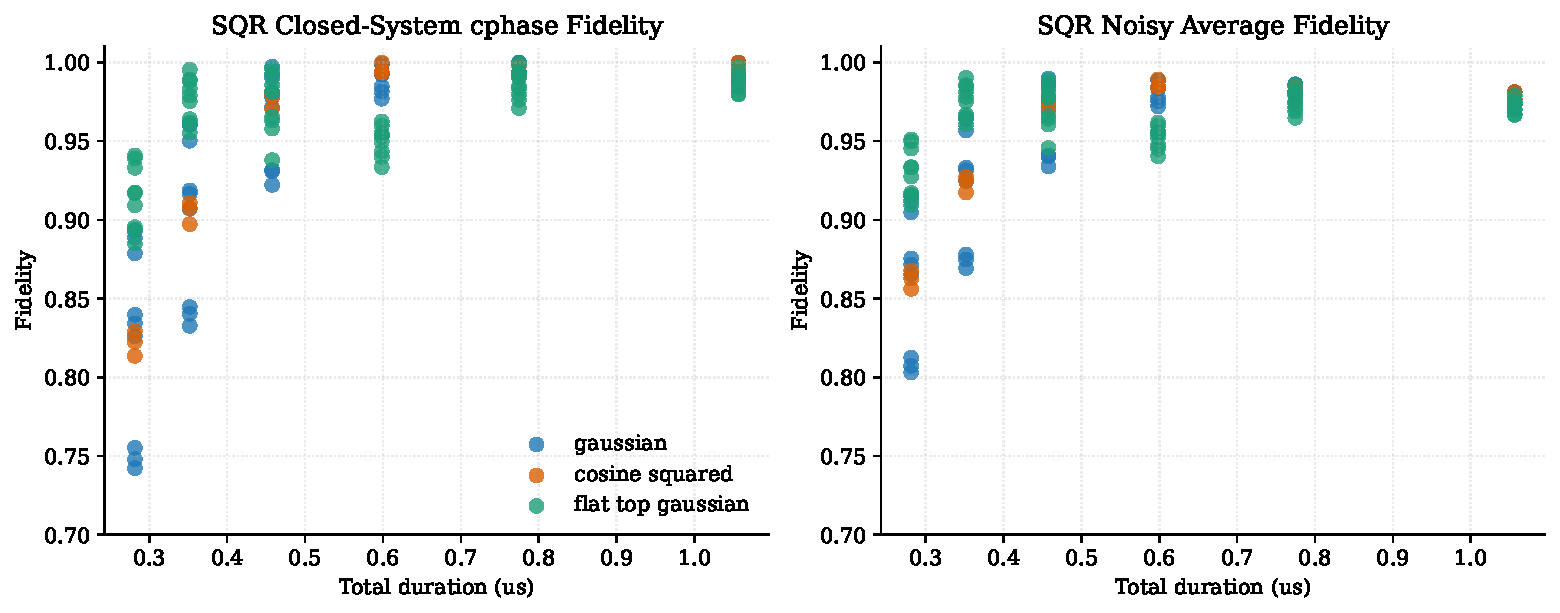
\includegraphics[width=0.95\linewidth]{../figures/sqr_family_scan.pdf}
  \caption{Closed-system and noisy SQR performance for the literature-informed pulse families. Gaussian and cosine-squared pulses dominate the long-duration closed-system regime, while the best noisy operating point shifts to a shorter flat-top Gaussian pulse. Horizontal structure in the noisy panel reflects the fact that several shape and amplitude variants cluster near the same practical fidelity.}
  \label{fig:sqr_scan}
\end{figure}

Two follow-up observations matter for downstream studies. First, the strict logical process fidelity of the best noisy SQR point is only $0.892$, while the relaxed cphase metric is $0.990$. This confirms again that the physically relevant primitive is the cphase-relaxed one: a later virtual-$Z$ or SNAP cleanup layer is still needed when the application demands strict logical gauge. Second, the best noisy point is exactly the shortest duration in the scan that still resolves the $|\chi|/2\pi=\SI{2.84}{MHz}$ branch splitting well enough to keep spectator errors small.

\subsection{Geometric SNAP}

The geometric SNAP sequence is more demanding because it uses two selective $\pi$ pulses and therefore roughly doubles the selective-drive exposure. Even so, the literature prescription remains effective in the repository's standard parameter regime. The best closed and noisy SNAP points both occur for the flat-top Gaussian family at $|\chi|T_\pi/2\pi=2.2$, corresponding to two \SI{0.775}{\micro s} selective $\pi$ pulses and a total sequence duration \SI{1.549}{\micro s}. That point reaches closed process fidelity $0.9102$ and noisy average state fidelity $0.9377$.

The Gaussian-only SNAP family is only slightly worse, with closed fidelity $0.9010$ and noisy average fidelity $0.9331$ at the same duration scale. The main conclusion is therefore not that Gaussian is unusable, but that the flat-top plateau gives a small but consistent improvement at equal duration and equal number-resolution scale. Figure~\ref{fig:snap_scan} shows the full scan.

\begin{figure}[H]
  \centering
  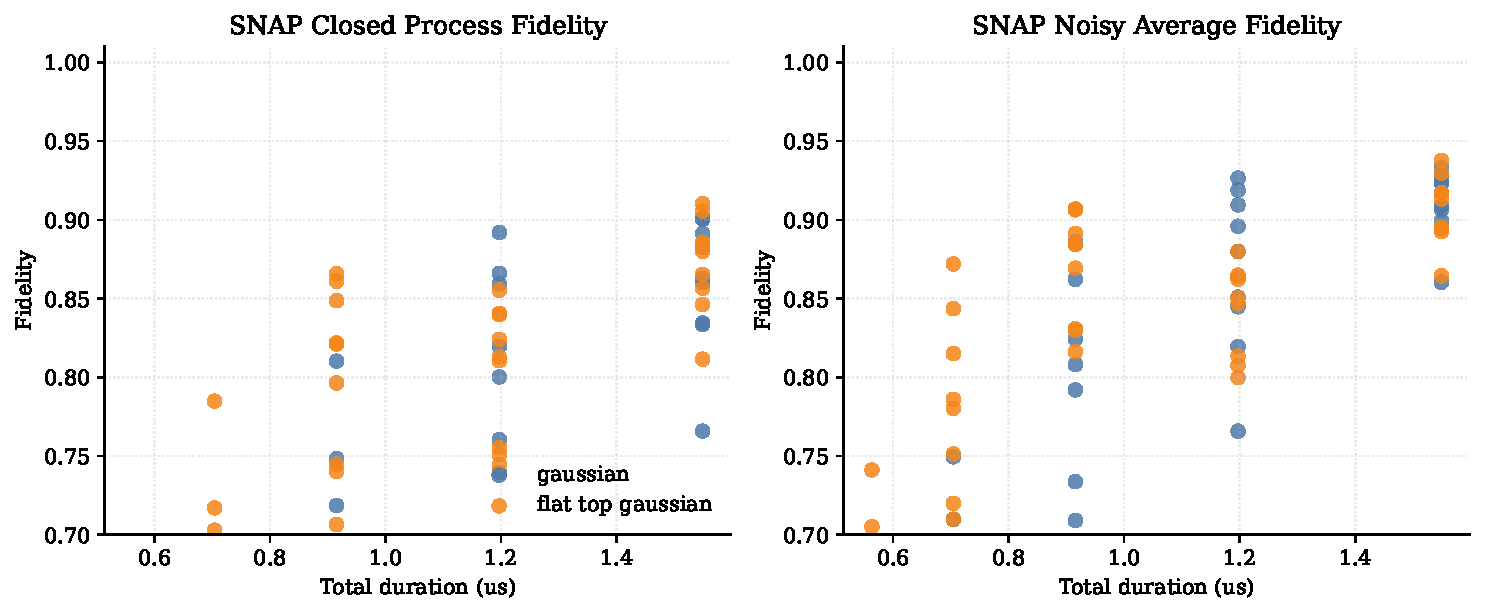
\includegraphics[width=0.95\linewidth]{../figures/snap_family_scan.pdf}
  \caption{Closed-system and noisy SNAP performance for Gaussian and flat-top Gaussian literature-style selective pulses. The best points occur once each selective $\pi$ pulse is long enough to resolve the number splitting but not so long that decoherence dominates.}
  \label{fig:snap_scan}
\end{figure}

Figure~\ref{fig:waveforms} collects the optimized noisy SQR and SNAP waveforms together with the best practical fidelities. The SQR optimum is visibly shorter and more compact, while the SNAP optimum retains the characteristic two-pulse structure of the geometric protocol.

\begin{figure}[H]
  \centering
  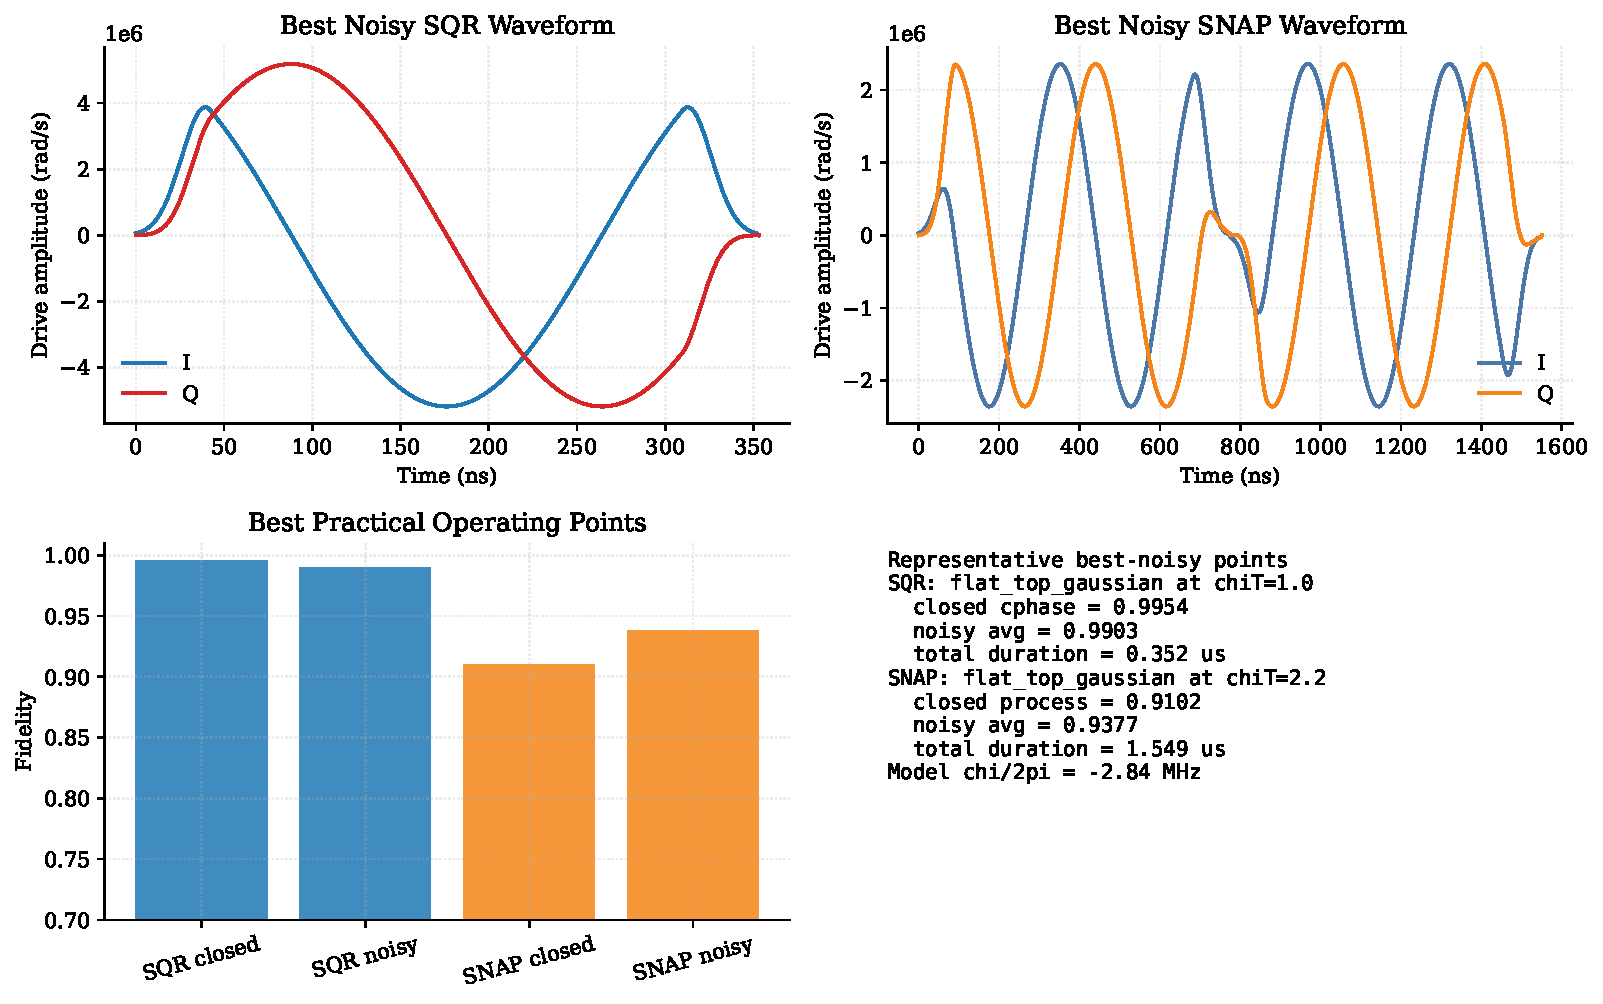
\includegraphics[width=0.95\linewidth]{../figures/best_waveforms_and_summary.pdf}
  \caption{Optimized noisy-reference waveforms and summary fidelities. The best noisy SQR point is a short flat-top Gaussian pulse at $|\chi|T/2\pi=1$, while the best SNAP point is a two-pulse flat-top Gaussian sequence at $|\chi|T_\pi/2\pi=2.2$.}
  \label{fig:waveforms}
\end{figure}

\section{Validation}

\subsection{Sanity Checks}

The validation suite confirms that the optimized pulses respect the expected limiting behavior. For the best SQR family, setting the target angle to zero preserves the computational basis with mean basis-state fidelity $1.0000$. For the best SNAP family, setting the target cavity phase to zero preserves the qubit-ground basis with mean basis-state fidelity $0.9982$. These checks verify that the pulse builders reduce to pure dispersive drift rather than introducing unintended swaps or excess leakage.

\subsection{Convergence Analysis}

Two numerical convergence checks were performed on the best noisy SQR and SNAP points. First, refining the time step from \SI{2}{ns} to \SI{1}{ns} changed the best noisy SQR fidelity by only $7.0\times 10^{-5}$ and the best noisy SNAP fidelity by $1.2\times 10^{-4}$. Second, increasing the storage cutoff from $n_\mathrm{cav}=7$ to $8$ changed the same fidelities by less than $5\times 10^{-7}$. These results show that the reported optima are not artifacts of the chosen discretization or cutoff.

\subsection{Literature Comparison}

Although this study does not reproduce one specific published hardware dataset, its optimized durations are quantitatively consistent with the number-selectivity rules reported in the literature. For the repository parameter $|\chi|/2\pi=\SI{2.84}{MHz}$, the basic selectivity scale is
\begin{equation}
\frac{1}{2|\chi|} \approx \SI{176}{ns}.
\end{equation}
The best noisy SQR point uses \SI{352}{ns}, the best closed Gaussian and cosine-squared SQR points use \SI{1.056}{\micro s}, and the best SNAP $\pi$ pulses use \SI{0.775}{\micro s}. Those are factors of roughly $2.0$, $6.0$, and $4.4$ above $1/(2|\chi|)$, respectively, which is exactly the long-pulse, number-resolved regime expected from the qcMAP and SNAP literature~\cite{leghtas2013qcmap,heeres2015snap,degraaf2025dualrail}.

\section{Discussion}

Three physical conclusions stand out. First, the best closed-system SQR pulses are not the best practical pulses under noise. Once transmon relaxation and dephasing are included, shorter flat-top Gaussian selective drives outperform the most selective long Gaussian or cosine-squared pulses because they pay less coherence cost while still resolving the photon-number splitting. This is the same qualitative tradeoff highlighted by the consolidated SQR study, but now tied directly to literature-style pulse families rather than to an internal family scan only.

Second, the cphase-relaxed metric remains the right figure of merit for selective qubit control. The best noisy SQR point achieves $0.9903$ average relaxed fidelity but only $0.892$ strict logical fidelity, meaning that most of the remaining imperfection is a branch-local phase issue, not a failure to perform the intended selective rotation. This supports the repository's current practice of treating ConditionalPhaseSQR as a natural primitive target and leaving strict-gauge cleanup to a later SNAP or virtual-$Z$ layer.

Third, geometric SNAP remains a viable but more expensive primitive in this parameter regime. Its best total duration is about four times the basic selectivity scale and about four times the best practical SQR duration. That is consistent with SNAP's role in the broader hybrid-control story: it is powerful for cavity-phase sculpting, but it is not the cheapest selective primitive when a relaxed SQR target is sufficient.

For experimental planning, that translates into a simple calibration order. Start from the short flat-top Gaussian SQR pulse if the near-term goal is branch-selective qubit action inside a larger control stack. Move to SNAP only when the experiment specifically needs an exact cavity phase layer or logical-gauge cleanup that cannot be absorbed into later virtual-$Z$ corrections. The literature-informed duration scales reported here are therefore best viewed as realistic first guesses for hardware calibration, not merely as simulation optima.

\section{Conclusion}

This study turns the literature pulse prescriptions for selective qubit rotation and SNAP into a validated, repository-native reference dataset. Gaussian and cosine-squared selective pulses retain the highest closed-system SQR performance near $|\chi|T/2\pi=3$, but the best noisy SQR point is a shorter flat-top Gaussian pulse at $|\chi|T/2\pi=1$ with relaxed-fidelity $0.9903$. For SNAP, the best point is a flat-top Gaussian two-$\pi$ sequence at $|\chi|T_\pi/2\pi=2.2$, reaching closed process fidelity $0.910$ and noisy average fidelity $0.938$. These results provide a concrete pulse-level handoff for the repository's existing SQR and hybrid-control studies.

For an experimentalist, the actionable message is to treat short flat-top Gaussian SQR as the default selective primitive at the repository's standard operating point, and to use flat-top Gaussian SNAP as the follow-on cavity-phase tool when exact gauge control is worth the extra sequence time.

\section{Limitations and Future Work}

\subsection{Known Limitations}

The first limitation is architectural: \texttt{cqed\_sim} still lacks first-class pulse builders and waveform-bridge coverage for \texttt{SNAP} and \texttt{ConditionalPhaseSQR}. This study therefore implements those waveform families locally, which is scientifically acceptable but not yet the cleanest reusable software path.

The second limitation is the noise model. The replay uses representative but not device-calibrated relaxation, dephasing, and storage thermal occupation. The reported optima are therefore best viewed as realistic reference points for the repository's standard parameter regime, not as direct predictions for one measured chip.

The third limitation is scope. The study uses a qubit-plus-storage model with a fixed logical window $n=0,\ldots,3$. It does not include explicit readout-mode backaction, cat-code logical subspaces, or direct open-system optimal control.

\subsection{Suggested Improvements}

\begin{itemize}
  \item \textbf{[P1 | HIGH]} Upstream the study-local builders into \texttt{cqed\_sim}. Native support for literature-style selective Gaussian, flat-top Gaussian, \texttt{SNAP}, and \texttt{ConditionalPhaseSQR} would remove the current duplication and make downstream hybrid-control studies cleaner.
  \item \textbf{[P2 | MEDIUM]} Replay the best SQR and SNAP points in a three-mode qubit-storage-readout model. This is the most direct next step for studies that already rely on explicit readout noise or concurrent readout.
  \item \textbf{[P2 | MEDIUM]} Re-optimize the same pulse families with an explicit multilevel transmon objective that reports both logical fidelity and $|f\rangle$ leakage during optimization rather than only during replay.
  \item \textbf{[P2 | LOW]} Swap the representative noise point for a device-calibrated noise import when one becomes available, then regenerate the duration scans and the recommendation table.
  \item \textbf{[P3 | HIGH]} Extend the same literature-informed pulse definitions to cat and binomial logical encodings, where the best balance between SQR and SNAP may change.
\end{itemize}

\subsection{Open Questions}

The most immediate open question is whether the flat-top advantage found here survives once readout-induced backaction is included explicitly. A second question is how much of the remaining strict-gauge SQR error can be removed by a short appended SNAP cleanup layer without erasing the noisy-duration advantage of the flat-top SQR pulse. Finally, it remains to be tested whether the same pulse hierarchy survives in larger logical windows, where $\chi'$ and Kerr will make long waits and long selective pulses increasingly nonlinear across photon number.

\bibliographystyle{unsrtnat}
\bibliography{references}

\end{document}
